\documentclass[../main.tex]{subfiles}
\graphicspath{
    {"../img/"}
    {"img/"}
}

\begin{document}
    \begin{large}
        końcówka dowodu:
    \end{large}

    \begin{figure}
        \centering
        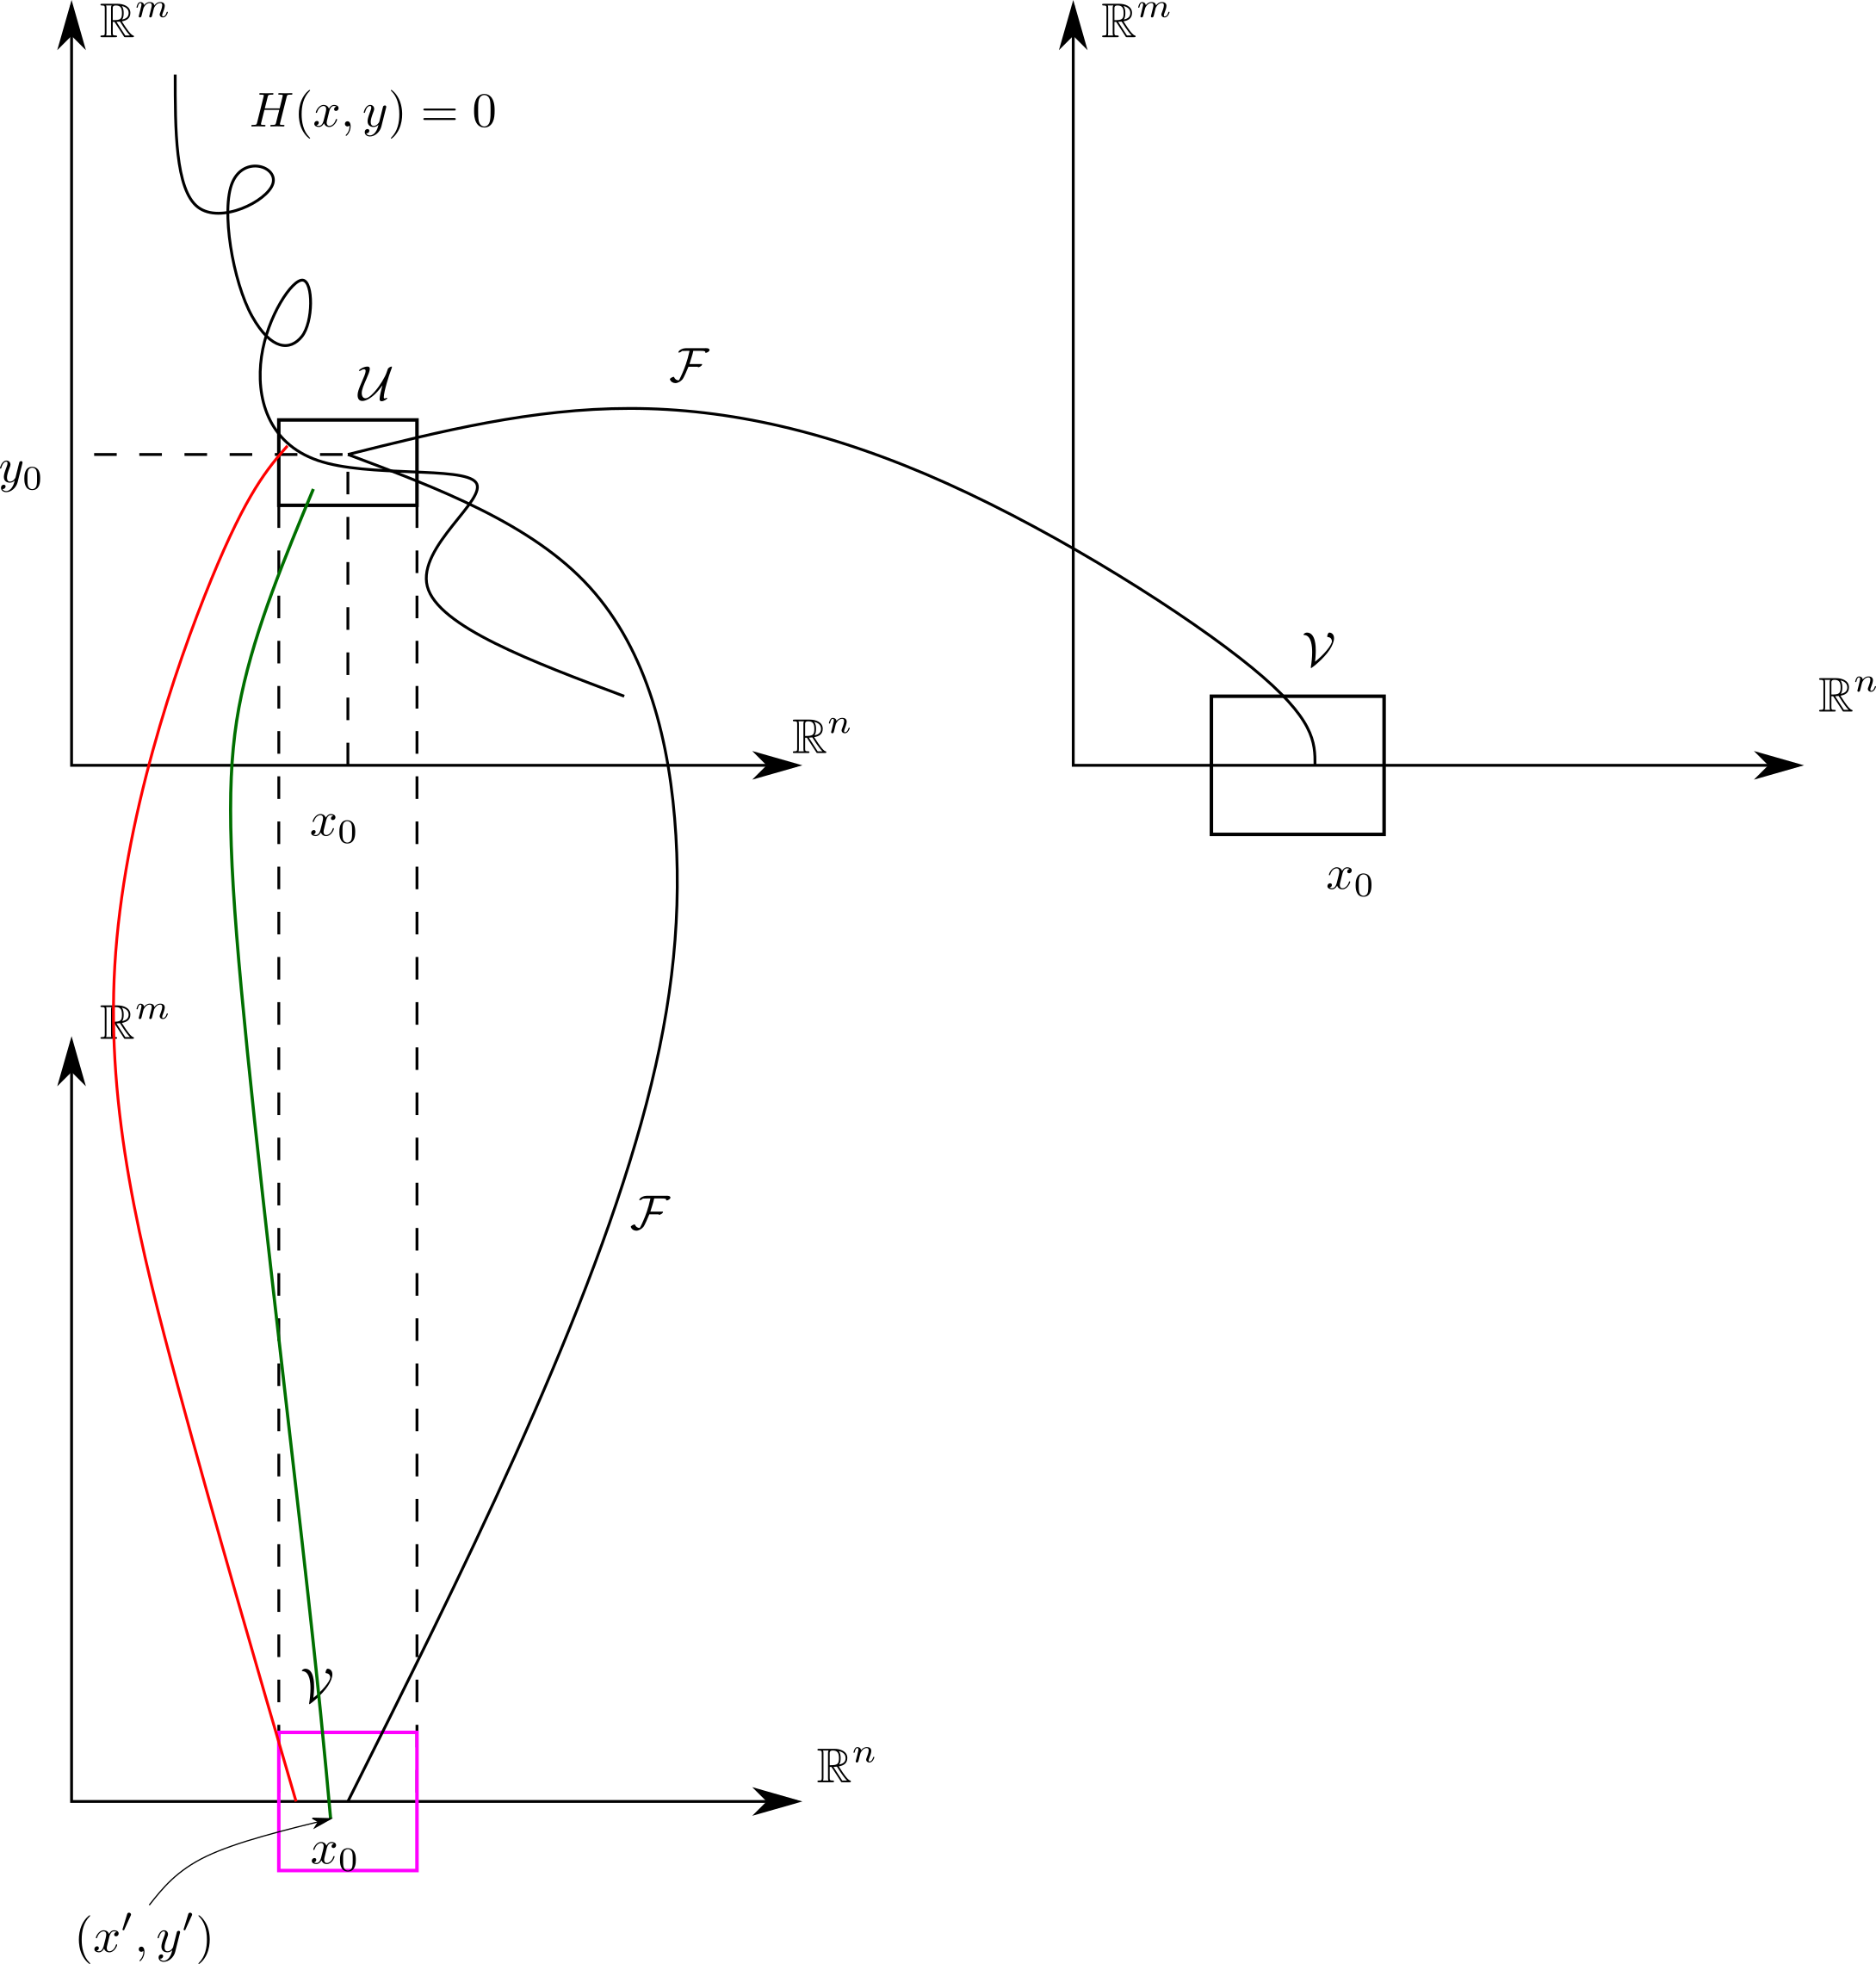
\includegraphics[width=\textwidth]{fig_21}
        \caption{}
        \label{fig:fig_21}
    \end{figure}

    Dla $(x',y')\in \mathcal{V},$
    \[
        F^{-1}(x',y') = (a(x',y'),b(x',y'))
    .\]
    Wiemy, że $a: \mathbb{R}^{n+m}\to\mathbb{R}^{n}$ i $b: \mathbb{R}^{n+m}\to\mathbb{R}^m$ istnieją i są różniczkowalne, bo $F^{-1}$ istnieje. Co jeszcze wiemy o funkcjach $a$ i $b$?\\
    Wiemy że  \[
        (x',y') = F(F^{-1}(x',y') = F(\underbrace{a(x',y')}_{n} , \underbrace{b(x',y')}_{m})
    .\]
    Oznacza to, że
    \[
        a(x',y') = x'
    .\]
    Czyli $a(x',y')$ jest identycznością, czyli:
    \[
        (x',y') = F(x',b(x',y')) \implies x'=x \implies (x,y') = F(x,b(x,y'))
    .\]
    Czyli jeżeli $y=b(x,0)$, to wtedy
    \[
        F(x,y) = (x,0)\text{, czyli } (x,H(x,y)) = (x,0)
    .\]
    Czyli dla $y = (x,0)$ otrzymujemy, że
    \[
        H(x,y)=0
    .\]
    Jeżeli oznaczymy $b(x,0) \overset{\text{ozn}}{=} \varphi(x)$, to znaczy, że znaleźliśmy funkcję $\varphi(x), \varphi:\mathbb{R}^n\to\mathbb{R}^m$ taką, że \[
        H(x,\varphi(x))=0 \quad\Box
    .\]

    \begin{definicja}
        Ekstrema związane\\

    \end{definicja}
    przykład:
    \[
        f(x,y) = x+y,\quad G(x,y) = (x-1)^1 + (y-1)^2 - 1,\quad M= \left \{ (x,y)\in\mathbb{R}^2,G(x,y) = 0\right \}
    .\]
    Szukamy minimum lub maksimum $f$ na $M$
    \begin{figure}
        \centering
        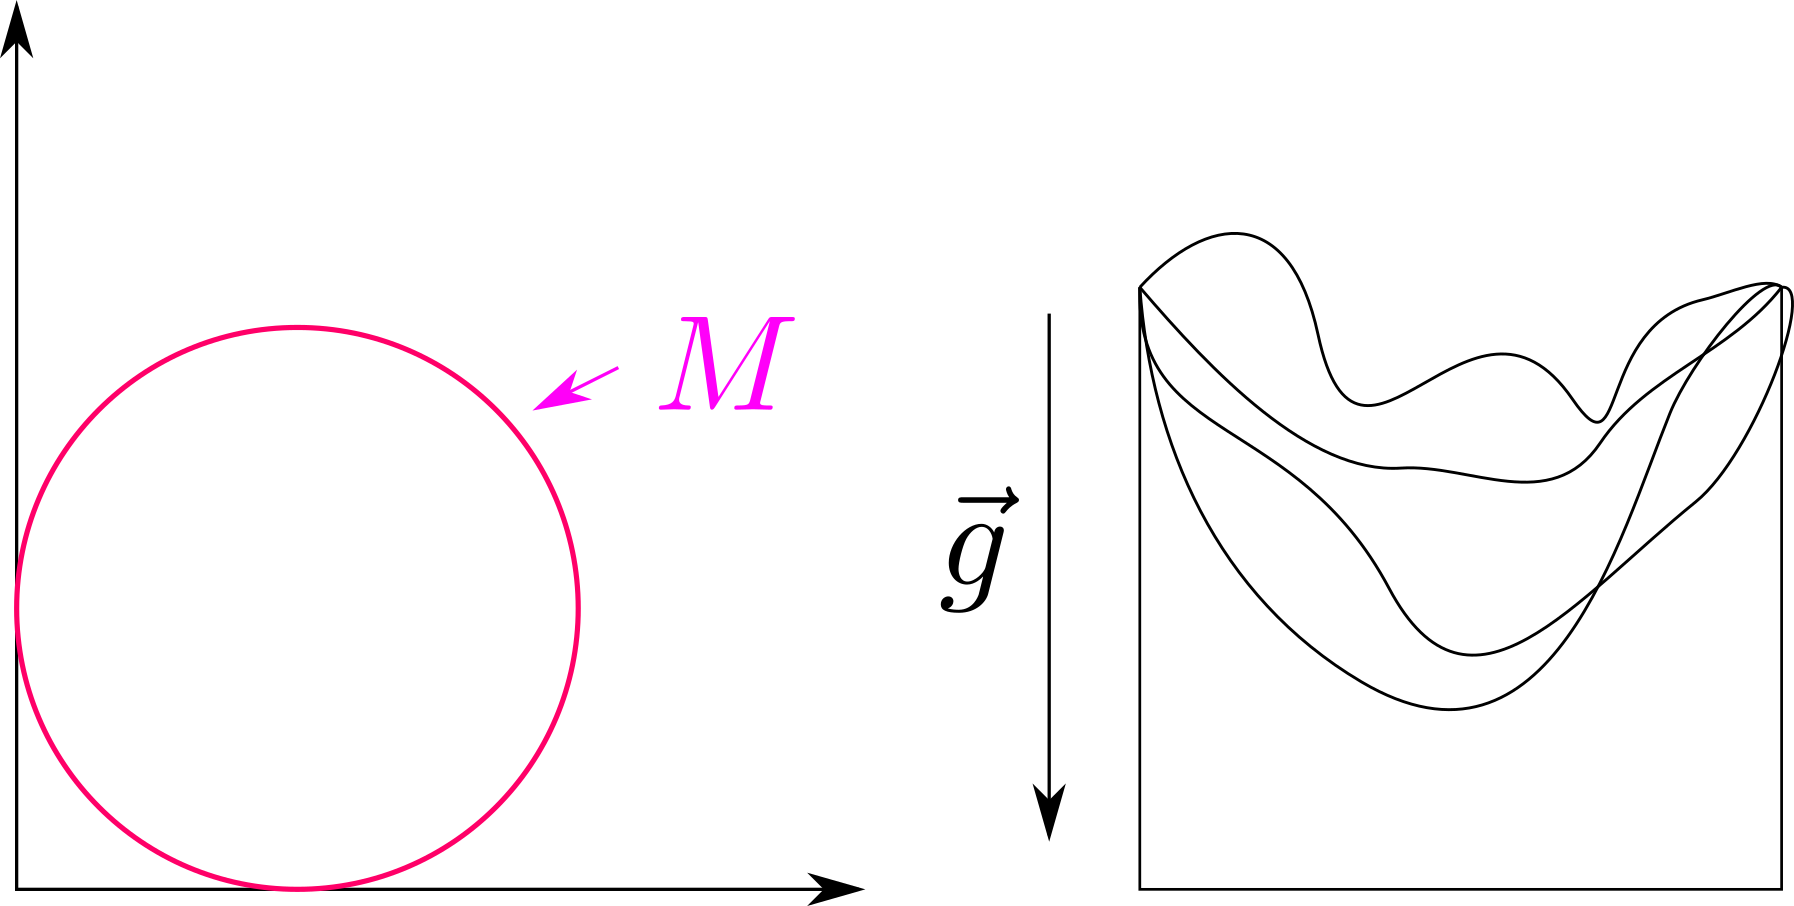
\includegraphics[width=0.8\textwidth]{fig_22}
        \caption{$G(x,y)$ i sznurek o stałej długości w polu grawitacyjnym}
        \label{fig:fig_22}
    \end{figure}

    Rozważmy linię o stałej wartości $x+y$
    \begin{figure}
        \centering
        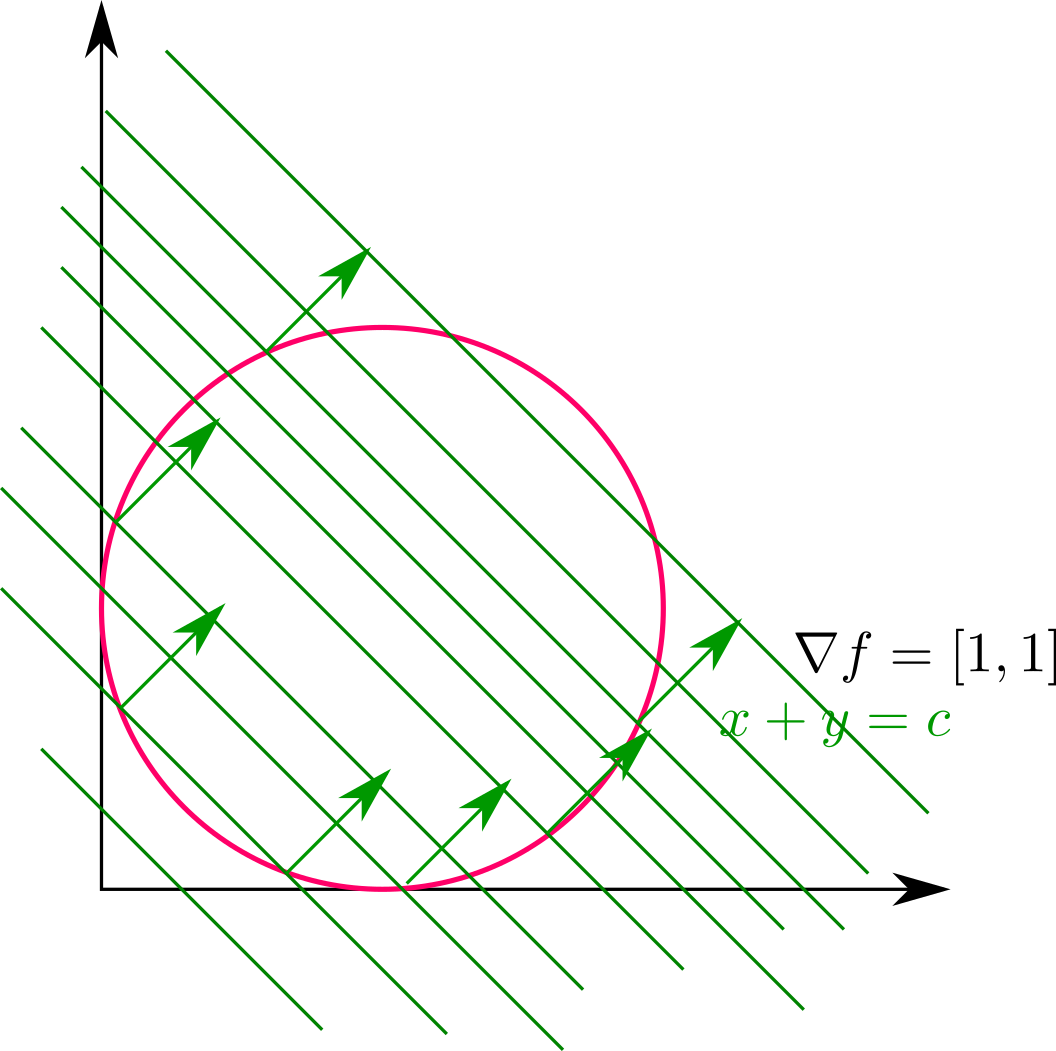
\includegraphics[width=0.7\textwidth]{fig_23}
        \caption{Biedronka łazi po obręczy rowerowej z włączonym wentylatorem, gdzie wyląduje???}
        \label{fig:fig_23}
    \end{figure}

    \begin{definicja}
        Niech $f:\mathbb{R}^{n}\to\mathbb{R}^1$ i $M\subset \mathbb{R}^n$ - zbiór.\\
        Mówimy, że $f$ ma minimum/maksimum związane na zbiorze $M$, w punkcie $x_0\in M$, jeżeli
        \[
            \underset{r}{\exists} \underset{\substack{h\\  \Vert h \Vert < r \\ (x_0+h)\in M}}{\forall} f(x_0+h)\leq f(x_0)
    .\]
    \end{definicja}
    \begin{figure}
        \centering
        \includegraphics[width=0.6\textwidth]{fig_24}
        \caption{}
        \label{fig:fig_24}
    \end{figure}

    \begin{large}
        Ekstrema związane podejście I\\
    \end{large}

    \vspace{1cm}

    Niech $f(x,y):\mathbb{R}^2\to\mathbb{R}^1$ \\
    $G(x,y): \mathbb{R}^2\to\mathbb{R}^1$\\
    $M = \left\{ (x,y), G(x,y) = 0 \right\} $
    Szukamy minimum/maksimum $f$. Można wyliczyć $y(x)$ z więzów, wstawić do $f$ i zbadać ekstrema funkcji jednej zmiennej $g(x) = f(x,y(x))$.
    Kiedy nie umiemy wyliczyć $y(x)$ z więzów, możemy założyć, że $y(x)$ jednak istnieje i $G(x,y(x)) = 0$. Wtedy:
    \[
    \frac{\partial G}{\partial x} + \frac{\partial G}{\partial y} \frac{\partial y}{\partial x} = 0
    .\]
    \[
        \frac{\partial y}{\partial x}  = - \frac{\frac{\partial G}{\partial x}}{\frac{\partial G}{\partial y} }
    .\]

    \[
        \text{czyli: } g'(x) = \frac{\partial f}{\partial x} + \frac{\partial f}{\partial y} \frac{\partial y}{\partial x} = 0
    .\]
    \[
        \frac{\partial f}{\partial x} + \frac{\partial f}{\partial y} \frac{-\frac{\partial G}{\partial x}}{\frac{\partial G}{\partial y} } = 0
        \implies \underline{\frac{\partial G}{\partial y} \frac{\partial f}{\partial x} = \frac{\partial f}{\partial y} \frac{\partial G}{\partial x}}
    .\]

    A co by było, gdyby $G(x,y) = 0$ zadawał funkcję $x(y)$?\\
    \[
        G(x(y),y) = 0
    .\]
    Czyli badalibyśmy wtedy funkcję \[
        P(y) = f(x(y),y)\quad P'(y) = 0 \implies \frac{\partial f}{\partial x} \frac{\partial x}{\partial y} + \frac{\partial f}{\partial y}  = 0
    .\]
    ale
    \begin{equation}\label{eq:eqx}
        \frac{\partial x}{\partial y}  = - \frac{\frac{\partial G}{\partial y}}{\frac{\partial G}{\partial x}} \implies \frac{\partial f}{\partial x} \frac{-\frac{\partial G}{\partial y} }{\frac{\partial G}{\partial x} }+\frac{\partial f}{\partial y} = 0 \implies \frac{\partial f}{\partial x} \frac{\partial G}{\partial y} = \frac{\partial f}{\partial y} \frac{\partial G}{\partial x}
    \end{equation}

    Co oznacza warunek \ref{eq:eqx}?\\
    Wiemy, że
    \[
        f' = \left[ \frac{\partial f}{\partial x} , \frac{\partial f}{\partial y}  \right] G' = \left[ \frac{\partial G}{\partial x} , \frac{\partial G}{\partial y}  \right]\text{, czyli}
    .\]
    \[
        V = \left[ A,B \right] \quad W = \left[ C,D \right] \text{ i } AD = BC
    .\]
    \[
    \frac{A}{B} = \frac{C}{D} = \lambda\in \mathbb{R}
    .\]
    Stąd wiadomo, że \[
    A = B\lambda, \quad C = D\lambda
    .\]
    \[
        V = \left[ B\lambda, B \right] ,\quad B = \left[ \lambda, 1 \right], \quad W = \left[ D\lambda, D \right], \quad D = \left[ \lambda, 1 \right]
    .\]
    Czyli warunek na to,  aby $G'(x) = 0$, albo  $P'(y) = 0$ oznacza, że \[
        \underset{\substack{\lambda\in\mathbb{R}\\ \lambda\neq 0}}{\exists} f' = \lambda G',  \quad G(x,y) = C
    .\]
    \begin{equation}\label{eq:eqy}
    \quad \frac{\partial f}{\partial x} - \lambda \frac{\partial G}{\partial x} = 0, \quad \frac{\partial f}{\partial y} - \lambda \frac{\partial G}{\partial y} = 0
    \end{equation}
    Wielkość $\lambda$ często nazywa się \textit{mnożnikiem Lagrange}

    \begin{obserwacja}
        Do warunku (\ref{eq:eqy}) można dojść na sktóry przez funkcję $H(x,y) = f(x,y) - \lambda G(x,y)$ i badanie $H(x,y)$ tak, jakby była to funkcja $\mathbb{R}^2\to \mathbb{R}^1$ bez żadnych więzów.\\
        \[
            \frac{\partial H}{\partial x} = 0, \quad \frac{\partial H}{\partial y} = 0 \left( \text{ + warunek } G(x,y) = 0 \right)
        .\]
    \end{obserwacja}
    \begin{pytanie}
        Co ze zbadaniem $G''(x)$ lub $P''(y)$?\\
        Odpowiedź: lepiej inaczej\ldots (XD), to znaczy, potrzebujemy nowego języka.
    \end{pytanie}

    Przy liczeniu ekstremów funkcji jednej zmiennej badaliśmy \[
        f(x_0+h) - f(x_0) \tilde = f''(x_0)(h,h)
    .\]

    \begin{figure}
        \centering
        \includegraphics[width=0.8\textwidth]{fig_25}
        \caption{}
        \label{fig:fig_25}
    \end{figure}

\end{document}
